\documentclass[journal]{IEEEtran}

\usepackage{amsmath,amsfonts,amssymb}
\usepackage{booktabs}
\usepackage{graphicx}
\usepackage{multirow}
\usepackage{textcomp}
\usepackage{xcolor}
\usepackage{url}
\usepackage{cite}
\usepackage[hidelinks]{hyperref}

\title{Metric Divergence and Anti-Gaming Diagnostics for Streaming Acoustic Echo Cancellation}

\author{Bozhong Liu%
\thanks{Bozhong Liu is an independent researcher. Email: \texttt{bliu012@e.ntu.edu.sg}. ORCID: 0009-0007-5023-0655.}}

\markboth{IEEE Transactions on Audio, Speech and Language Processing}%
{Liu: Metric Divergence and Anti-Gaming Diagnostics for Streaming AEC}

\begin{document}

\maketitle

\begin{abstract}
Streaming acoustic echo cancellation (AEC) is commonly evaluated through intrusive reconstruction metrics, no-reference blind metrics, and subjective listening scores, but these axes can disagree under double-talk and aggressive suppression. This paper presents a harmonized 16~kHz diagnostic evaluation protocol for streaming AEC systems, combining matched intrusive scale-invariant signal-to-distortion ratio (SI-SDR) evaluation, blind AECMOS scoring, microphone-active frame retention analysis, anti-gaming validation controls, and returned item-level listening summaries. As a case study, we evaluate a support-conditioned acoustic echo cancellation (SC-AEC) causal probe that injects online statistics from a causal linear echo estimate into a compact residual suppressor. Under the shared objective protocol, a retrained public ASTWS architecture (ASTWS-H16k) outperforms the support-conditioned SC-AEC-Echo point on clean, noisy, and low signal-to-echo ratio (low-SER) SI-SDR, reaching 11.71, 9.08, and 7.57~dB versus 7.55, 6.94, and 3.10~dB. On the official ICASSP~2023 blind set, SC-AEC-Echo obtains a higher AECMOS-Echo coordinate than ASTWS-H16k, but retention diagnostics and validation controls show that this coordinate is not reliable as standalone perceptual evidence: an all-zero output receives high AECMOS scores in the diagnostic suite. Returned 72-base item-level listening summaries further indicate that the echo-oriented coordinate does not translate into the strongest overall MOS or acceptability. The resulting contribution is a claim-boundary framework for streaming AEC evaluation: no-reference echo metrics should be paired with retention diagnostics, anti-gaming controls, and perceptual anchors before supporting method claims.
\end{abstract}

\begin{IEEEkeywords}
acoustic echo cancellation, streaming speech enhancement, double-talk robustness, no-reference evaluation, anti-gaming diagnostics
\end{IEEEkeywords}

\section{Introduction}
\IEEEPARstart{S}{treaming} acoustic echo cancellation remains hard because the deployment target is defined by competing requirements rather than by one metric: low algorithmic latency, time-varying echo paths, double-talk overlap, and tolerance to playback corruption. The recent challenge line made this tension explicit by combining synthetic intrusive evaluation with blind real-recording scoring under realistic latency limits~\cite{cutler2021aec,cutler2022aec,cutler2024aec}. A credible streaming study therefore needs more than a strong table row. It needs a shared evaluation contract, anti-gaming controls for no-reference metrics, and explicit boundaries on what each evidence source can support.

That need is still not met consistently. Public AEC results are often compared across partially mismatched pipelines: different sample rates, different waveform reconstruction paths, or different baseline wrappers. The resulting tables can be numerically impressive while remaining difficult to audit. Blind no-reference reporting is a second gap. A system can improve echo suppression by moving to a more aggressive overlap regime, while another system preserves near-end quality by remaining more conservative. Both behaviors matter and should be reported explicitly.

This paper treats a support-conditioned streaming AEC family as an exploratory diagnostic probe. The probe is built around online statistics derived from a causal linear echo estimate, then evaluated against retrained and classical comparators under one harmonized 16~kHz contract. Its purpose in this manuscript is not to introduce a deployable champion system, but to stress-test how intrusive metrics, blind no-reference coordinates, retention diagnostics, and returned listening summaries interact when a nonlinear suppressor moves toward aggressive echo removal.

The resulting evidence exposes a useful measurement hazard. Under the shared objective protocol, ASTWS-H16k is stronger on clean, noisy, and low-SER SI-SDR. On the official blind set, SC-AEC-Echo occupies a more echo-oriented AECMOS coordinate, but the all-zero validation control and microphone-active retention table show why that coordinate is unsafe in isolation. Returned item-level listening summaries further show that the echo-oriented coordinate does not translate into the strongest overall MOS or acceptability. This makes the diagnostic protocol itself the main object of the paper.

The paper makes three contributions:
\begin{enumerate}
    \item an evaluation contribution: a harmonized 16~kHz streaming AEC protocol with matched clean, noisy, low-SER, and blind diagnostic views;
    \item a diagnostic contribution: an AECMOS anti-gaming and retention analysis showing that high no-reference echo scores can coincide with degenerate or over-suppressed outputs;
    \item a claim-boundary contribution: a support-conditioned streaming AEC case study showing that family-level conditioning benefits do not imply cue-specific causality or preferred returned listening outcomes.
\end{enumerate}

\section{Related Work}
The recent AEC challenge series is the right benchmark context because it ties together synthetic evaluation, blind real-recording evaluation, and deployment-style latency constraints~\cite{cutler2021aec,cutler2022aec,cutler2024aec}. The 2023 challenge is especially relevant because it exposes both blind double-talk and blind far-end single-talk behavior, making it a better anchor for operating-point analysis than synthetic tables alone~\cite{cutler2024aec}.

Modern neural AEC systems now span three overlapping directions. The first direction is unified enhancement front ends that handle AEC together with denoising, dereverberation, or source separation~\cite{omalley2022frontend,eskimez2023personalized,ristea2023deepvqe}. These works motivate deployment-aware framing, but they do not directly answer how a compact streaming suppressor should be conditioned online when the linear path becomes unreliable.

The second direction emphasizes better alignment, echo-path modeling, and stronger control signals. Streaming cross-attention alignment addresses microphone-reference mismatch explicitly~\cite{chen2023sca}. Hybrid adaptive-filter and neural methods such as NeuralKalman also show why classical state estimation remains relevant under double-talk and echo-path change~\cite{zhang2023neuralkalman}. Deep Echo Path Modeling uses a more explicit path representation and is therefore an important public comparator for the present study~\cite{zhao2024deepecho}. Attention-enhanced short-time Wiener solution shows that carefully structured filtering cues can materially improve a compact streaming model~\cite{zhao2024astws}. More recent work has pushed both target design and compact deployment further: interference-aware joint AEC+NS targets explicitly reduce near-speech shadowing during overlap~\cite{khanagha2024interference}, and CAGCRN shows that a small cross-attention AEC+NS model can remain deployment-friendly~\cite{wang2025cagcrn}. The present work sits in this family of control-aware streaming systems, but it frames its conditioning signal explicitly as online support statistics rather than as semantic or externally measured room descriptors.

The third direction concerns perceptual evaluation. AECMOS was proposed to separate echo impairment from other degradations in a no-reference setting, which makes it useful for blind operating-point analysis~\cite{aecmos2021}. More general non-intrusive perceptual predictors such as DNSMOS P.835 and NISQA further show how modern communication-quality evaluation has moved toward multidimensional listener-facing scoring rather than a single intrusive distortion number~\cite{reddy2022dnsmosp835,mittag2021nisqa}. At the same time, broader speech-enhancement evaluations such as CHiME-7 UDASE showed that no-reference metrics and human judgments can diverge on real-domain data~\cite{udase2024eval}. That is why this paper uses blind no-reference scores as comparative operating-point evidence and treats the returned item-level listening summaries as the claim boundary for perceptual preference.

\section{Probe Architecture and Systems}
Rather than proposing the support-conditioned family as a deployable system, this section defines the diagnostic probe used to exercise the evaluation protocol. The architecture is expressive enough to expose an aggressive residual-suppression operating point, while the later destructive controls test whether the explicit support statistics carry cue-specific causal evidence.

\subsection{Streaming Setup}
Let $x_t$ denote the microphone waveform buffer and $r_t$ the far-end reference buffer at frame $t$. The system uses a 320-sample analysis window and a 160-sample hop at 16~kHz, corresponding to a 20~ms window and a 10~ms causal update interval. Short-time Fourier analysis produces
\begin{equation}
X_t, R_t \in \mathbb{C}^{F}, \qquad F = 161,
\end{equation}
with no future context. The model predicts an enhanced spectrum $\hat{S}_t$ and reconstructs the time-domain output through overlap-add synthesis.

\subsection{Online Support Statistics}
The control path is built from causal statistics that summarize what the linear echo estimate currently supports. Let $S_b \subset \{1,\ldots,F\}$ denote the $b$-th linear-frequency band in a uniform 12-way partition, and define the band reducer
\begin{equation}
\mathcal{B}(v)_b = \frac{1}{|S_b|}\sum_{f \in S_b} v_f.
\end{equation}
Using exponential smoothing factor $\lambda = 0.85$, the front end tracks
\begin{equation}
\tilde{C}_t = \lambda \tilde{C}_{t-1} + (1-\lambda)\mathcal{B}(X_t R_t^\ast),
\end{equation}
\begin{equation}
\begin{aligned}
\tilde{P}_t^r &= \lambda \tilde{P}_{t-1}^r + (1-\lambda)\mathcal{B}(|R_t|^2),\\
\tilde{P}_t^m &= \lambda \tilde{P}_{t-1}^m + (1-\lambda)\mathcal{B}(|X_t|^2).
\end{aligned}
\end{equation}
The 12-band complex support summary is
\begin{equation}
\mu_t = \frac{\tilde{C}_t}{\tilde{P}_t^r + \epsilon} \in \mathbb{C}^{12},
\end{equation}
and the corresponding band uncertainty summary is the complement of magnitude coherence:
\begin{equation}
u_t = 1 - \frac{|\tilde{C}_t|}{\sqrt{\tilde{P}_t^m \tilde{P}_t^r + \epsilon}}
\in [0,1]^{12}.
\end{equation}
These quantities behave like a compact online support estimate for the linear path, but they are not Bayesian posterior probabilities.
The corresponding linear echo estimate is a causal bandwise normalized cross-spectrum estimate, not a learned filter bank:
\begin{equation}
\hat{H}_{t,b}^{lin}=\frac{\tilde{C}_{t,b}}{\tilde{P}_{t,b}^{r}+\epsilon},
\qquad
\hat{E}^{lin}_{t,f}=\hat{H}^{lin}_{t,b(f)}R_{t,f}.
\end{equation}
The only state in this estimator is the exponentially smoothed cross-power and auto-power triplet
$(\tilde{C}_t,\tilde{P}_t^r,\tilde{P}_t^m)$; no future frame, offline alignment, or oracle echo path is used.

To describe coarse temporal mismatch, the front end also computes a 5-way delay distribution over candidate lags
\begin{equation}
\tau \in \{0,16,32,48,64\},
\end{equation}
using normalized frame-level correlation scores:
\begin{equation}
c_t(\tau) = \frac{\langle \mathbf{x}_t,\mathbf{r}_t^{(\tau)} \rangle}
{\|\mathbf{x}_t\|_2 \|\mathbf{r}_t^{(\tau)}\|_2 + \epsilon},
\qquad
d_t = \mathrm{softmax}_\tau(c_t(\tau)) \in \mathbb{R}^{5}.
\end{equation}
The lag candidates are samples at 16~kHz, i.e., $0$--$4$~ms. They are used as a coarse local alignment cue inside the causal support estimator, not as a full acoustic echo-path delay search.
The scalar speech-to-echo risk cue is derived from the balance between linear echo energy and residual energy:
\begin{equation}
E_t^{lin} = \frac{1}{F}\sum_f |\hat{E}_{t,f}^{lin}|^2, \qquad
E_t^{res} = \frac{1}{F}\sum_f |X_{t,f} - \hat{E}_{t,f}^{lin}|^2,
\end{equation}
\begin{equation}
\rho_t = \sigma \!\left( \log \!\left(1 + \frac{E_t^{res}}{E_t^{lin} + \epsilon}\right) \right).
\end{equation}

\subsection{Conditioned Residual Suppressor}
The complete control vector is
\begin{equation}
s_t = [\Re\mu_t, \Im\mu_t, u_t, d_t, \rho_t] \in \mathbb{R}^{42}.
\end{equation}
A two-layer MLP maps $s_t$ to a control representation $c_t \in \mathbb{R}^{192}$. The probe combines this control with residual features derived from the microphone, far-end reference, causal linear echo estimate, residual spectrum, log magnitudes, and residual-reference phase relation. Let $\hat{E}^{lin}_t$ denote the linear echo estimate and $\tilde{R}_t = X_t - \hat{E}^{lin}_t$ the residual spectrum before neural suppression. The residual feature vector is summarized as
\begin{equation}
v_t=[X_t,R_t,\hat{E}^{lin}_t,\tilde{R}_t,\log |X_t|,\log |R_t|,\log |\tilde{R}_t|,\Delta\phi_t],
\end{equation}
where $\Delta\phi_t$ contributes sine and cosine phase features. The residual stack, support vector, and control vector are projected into a recurrent suppressor with a single GRU cell. Conditioning enters twice: once before the recurrent backbone and once before the output heads,
\begin{align}
r_t &= \phi_r(v_t) \in \mathbb{R}^{224}, \nonumber\\
b_t &= \phi_s(s_t) \in \mathbb{R}^{224}, \nonumber\\
q_t &= \phi_q(c_t) \in \mathbb{R}^{224},
\end{align}
\begin{align}
g_t &= \phi_f([r_t, b_t, q_t]) \in \mathbb{R}^{256}, \nonumber\\
h_t &= \mathrm{GRUCell}(g_t, h_{t-1}).
\end{align}
Let $z_t = \phi_o(h_t)$ denote the post-backbone hidden feature. The evaluated family uses a head-side conditioning adapter
\begin{equation}
\tilde{z}_t = A(z_t, c_t),
\end{equation}
where $A(\cdot,\cdot)$ is either an additive ReZero adapter or a FiLM adapter. A second head projection $\phi_h(c_t)$ is concatenated before predicting a residual echo term, speech gain, and noise mask:
\begin{equation}
\bar{z}_t = [\tilde{z}_t, \phi_h(c_t)].
\end{equation}
\begin{align}
\hat{M}^{res}_{t,f} &= \tanh(W_r\bar{z}_t)_{f}, &
\hat{E}^{res}_{t,f} &= \hat{M}^{res}_{t,f}\tilde{R}_{t,f},\\
G_{t,f} &= \sigma(W_g\bar{z}_t)_f, &
N_{t,f} &= \sigma(W_n\bar{z}_t)_f.
\end{align}
With noise-mask attenuation strength $\eta$, the final gain is
\begin{equation}
\bar{G}_{t,f}=\mathrm{clip}\!\left(G_{t,f}(1-\eta N_{t,f}),0,1\right),
\end{equation}
and the enhanced spectrum is
\begin{equation}
\hat{S}_{t,f}=\bar{G}_{t,f}\left(\tilde{R}_{t,f}-\kappa\hat{E}^{res}_{t,f}\right),
\end{equation}
where $\eta$ and $\kappa$ define the fixed operating point used for the reported artifacts.

\subsection{Double-Talk-Aware Objective}
Training combines waveform, complex-domain, magnitude-domain, and double-talk-aware penalties:
\begin{equation}
\begin{aligned}
\mathcal{L} =\;&
\lambda_w \mathcal{L}_{wav}
+ \lambda_c \mathcal{L}_{cpx}
+ \lambda_m \mathcal{L}_{mag}
+ \lambda_s \mathcal{L}_{sdw}\\
&+ \lambda_\ell \mathcal{L}_{lin}
+ \lambda_r \mathcal{L}_{res}
+ \lambda_p \mathcal{L}_{cons}
+ \lambda_n \mathcal{L}_{noise}.
\end{aligned}
\end{equation}
For the selected objective operating point, the effective weights are
$\lambda_w=0.5$, $\lambda_c=1.0$, $\lambda_m=0.5$, $\lambda_s=0.25$,
$\lambda_\ell=0.35$, $\lambda_r=0.25$, $\lambda_p=0.05$, and $\lambda_n=0.05$.
The family ablation reported later fixes this objective, so the additive-versus-FiLM ordering in the main paper is not explained by re-tuning loss weights across rows.

Here $\mathcal{L}_{wav}$ is waveform-domain $L_1$ error on the reconstructed near-end signal, $\mathcal{L}_{cpx}$ is real/imaginary STFT $L_1$ error, and $\mathcal{L}_{mag}$ is magnitude STFT $L_1$ error. $\mathcal{L}_{sdw}$ is the near-end speech-distortion-weighted term on active speech frames. $\mathcal{L}_{lin}$ penalizes residual echo left by the causal linear estimate, $\mathcal{L}_{res}$ penalizes residual echo left by the learned residual path, $\mathcal{L}_{cons}$ regularizes support-conditioned head behavior across adjacent frames, and $\mathcal{L}_{noise}$ is the auxiliary noise-mask target. The training target is clean near-end speech in the synthetic protocol and echo-free microphone speech in noisy variants. Double-talk-aware terms use clean near-end activity and echo activity from the manifest supervision; clean-speech active frames receive the speech-distortion emphasis, while far-end-dominant frames receive residual-echo emphasis.

SC-AEC-Echo uses the harmonized clean training manifest with 9,025 train and 475 validation examples, plus fixed validation and paper-test manifests containing 500 clean, 500 noisy, and 152 low-SER examples. It uses AdamW with learning rate $3\times10^{-4}$, weight decay $10^{-5}$, gradient clipping at $5.0$, seed $7$, batch size 128 in the reported artifact, and validation after every epoch. The selected SC-AEC-Echo point is the fixed seed-7 validation checkpoint selected at epoch 4 under the same streaming and runtime contract. SC-AEC-Preserve and SC-AEC-NoCond are reported as fixed companion identities from the same artifact family; this is a fixed-seed diagnostic artifact study, not a multi-seed stability claim.

\begin{table}[t]
\caption{SC-AEC-Echo training recipe. The row is reported as a fixed artifact recipe rather than as a multi-seed stability claim.}
\label{tab:scaec-recipe}
\centering
\small
\begin{tabular}{p{0.23\columnwidth}p{0.60\columnwidth}}
\hline
Item & Recipe detail \\
\hline
Data & 9025 train / 475 validation / 500 clean test / 152 low-SER test examples \\
Sample rate and target & 16 kHz, clean near-end speech target \\
Seed and scope & seed 7; single fixed-seed artifact study \\
Optimizer & AdamW, LR $3\times 10^{-4}$, weight decay $10^{-5}$, gradient clip 5.0 \\
Batch / accumulation & batch 128; gradient accumulation not recorded in artifact metadata \\
Training length & reported artifact completed 4 epochs / 284 optimizer steps; selected epoch 4 \\
Selection rule & best validation SI-SDR under the same streaming contract \\
Loss weights & $0.5L_{wav}+1.0L_{cpx}+0.5L_{mag}+0.25L_{sdw}+0.35L_{lin}+0.25L_{res}+0.05L_{cons}+0.05L_{noise}$ \\
\hline
\end{tabular}
\end{table}


\section{Diagnostic Evaluation Protocol}
\subsection{Evaluation Tracks and Claim Gates}
The protocol separates four evidence tracks. The intrusive track reports scale-invariant signal-to-distortion ratio (SI-SDR, dB), segmental signal-to-noise ratio (SegSNR, dB), echo return loss enhancement (ERLE, dB), double-talk preservation, and double-talk suppression only on matched examples with available targets. The blind no-reference track reports AECMOS only as an operating-point coordinate and requires anti-gaming controls. The retention track measures microphone-active frame dropout on blind double-talk clips so that aggressive suppression is visible even when no clean near-end target exists. The listening track uses returned item-level summaries only as perceptual boundary evidence because raw individual-rater rows are unavailable.

The same protocol also defines method-claim gates. Capacity and conditioning controls can support a family-level statement that an explicit conditioning path stabilizes this backbone under the reported recipe. Destructive support controls are required before attributing gains to specific cues. In the results below, these gates establish the evaluation boundary: cue-specific causality is not established, formal P.808 ranking is not claimed, and no-reference AECMOS is not treated as standalone perceptual evidence.

\subsection{Harmonized 16~kHz Evaluation Framework}
All primary objective claims are made under one harmonized 16~kHz streaming contract. The clean main table uses the harmonized synthetic public test split with 500 matched examples. The noisy table reuses the same example identity set under deterministic public-noise augmentation, also with 500 matched examples. The low-SER stress subset contains 152 matched double-talk-heavy examples and is used as the main overlap-robustness slice.

Every runnable system is evaluated through the same waveform path, sample rate, overlap-add reconstruction contract, and metric implementation. The main claim is therefore restricted to same-dataset, same-latency, same-metric comparison.

\subsection{Causality and Delay Accounting}
The model uses a 320-sample Hann analysis window and a 160-sample hop at 16~kHz. STFT analysis is computed with \texttt{center=false} semantics: each output frame is formed after the current 20~ms analysis buffer is available, and the recurrent state uses only the previous hidden state and previous support-estimator state. Streaming synthesis uses overlap-add with the same hop; it does not request future neural context. The practical algorithmic buffering delay is therefore one analysis window, 20~ms, with 10~ms frame updates. The far-end reference and microphone frame supplied at step $t$ are aligned at the same sample time before the local 0--4~ms delay-cue candidates are evaluated.

\subsection{Systems and Comparison Boundary}
The main paper-level public-architecture comparator is ASTWS-H16k, obtained by retraining the public ASTWS architecture under the declared harmonized 16~kHz recipe. Additional training safeguards were used only to make that public-baseline retraining finite and reproducible, and they are reported as baseline recipe details rather than hidden tuning. The original ASTWS and Deep Echo public checkpoints are retained as transfer-protocol audit rows rather than as primary baselines, because their public checkpoints do not reproduce their native reported regimes under this contract. A historical ICASSP~2022 baseline row is retained only as an appendix anchor. The support-conditioned family is represented by three frozen identities: SC-AEC-Echo for objective and blind echo-oriented analysis, SC-AEC-Preserve for preservation-biased listening analysis, and SC-AEC-NoCond for ablation only. SC-AEC-Echo uses approximately 1.79M parameters, compared with roughly 0.15M for ASTWS-H16k and ASTWS public-checkpoint transfer and 0.12M for Deep Echo public-checkpoint transfer under the same parameter-count procedure. A single-stream, batch-one latency harness estimates about 167.6M multiply-accumulates for this point. Parameter efficiency is therefore outside the positive evidence boundary; the SC-AEC row is retained for diagnostic contrast.

The NLMS row is a classical diagnostic baseline, not an optimized challenge system. It uses a deterministic 1024-tap normalized LMS filter at 16~kHz with step size 0.25, regularization $10^{-6}$, leakage 0, reference-energy floor $10^{-10}$, and the same aligned microphone/reference waveform path as the other systems. It applies no neural suppression, no validation tuning, and no explicit double-talk protection; this makes it auditable as a linear-path anchor but not competitive as a tuned modern AEC system.

\begin{table*}[t]
\caption{ASTWS-H16k retraining recipe and comparison boundary. Additional training safeguards were used only to make the public ASTWS architecture retrain finite under the harmonized 16 kHz recipe; they are reported as baseline recipe details.}
\label{tab:astws-recipe}
\centering
\small
\begin{tabular}{p{0.15\textwidth}p{0.36\textwidth}p{0.36\textwidth}}
\hline
Item & SC-AEC-Echo & ASTWS-H16k \\
\hline
Architecture & SC-AEC residual suppressor & Public ASTWS architecture \\
Train/validation data & Harmonized 16 kHz public train/val slices & Same harmonized 16 kHz train/val slices \\
Target & Clean near-end speech & Clean near-end speech \\
Optimizer & AdamW, LR $3\times10^{-4}$ & AdamW, LR 1e-4 \\
Training scale & seed 7, fixed single-seed artifact study & single retraining run \\
Batch / accumulation & batch-first waveform training & batch 1, accum. 8 \\
Loss & waveform, complex, magnitude, SDW, linear/residual consistency & SI-SDR, waveform L1, STFT mag/RI (0.25/0.5/1.0/0.25) \\
Training safeguards & none beyond family objective & warmup 500, grad clip 1.0, nonfinite skip rate 0.0006 \\
Selection & validation SI-SDR under streaming contract & validation SI-SDR, best epoch 6 \\
Fingerprint & reported in artifact metadata & sha256 57e00339b211... \\
\hline
\end{tabular}
\end{table*}


Real-time factor (RTF) is reported from the same timing protocol: single-stream inference, batch size one, one warm-up pass, repeated steady-state timing on one local workstation using PyTorch eager inference, and values rounded to two decimals, with rows below 0.01 reported as ``<0.01.'' The latency column is therefore a deployment-oriented comparator, not a hardware-independent throughput claim.

Fig.~\ref{fig:architecture} summarizes the signal path, support-statistics front end, and the two conditioning injection sites used by the support-conditioned family.

\subsection{Baseline Fidelity and Protocol Validation}
The public-checkpoint transfer rows require explicit fidelity discussion. We therefore separate four views: representative native reported numbers from the original public papers, native-compatible forward evaluation on a 128-example diagnostic probe, public-checkpoint transfer under the harmonized contract, and ASTWS-H16k as a retrained public-architecture row. The native-compatible forward path and corrected shared evaluation path agree exactly on the clean probe for ASTWS public-checkpoint transfer and Deep Echo public-checkpoint transfer, and a compact follow-up audit on the 152-example low-SER probe also yields zero waveform-path deltas for signal-to-distortion ratio and double-talk suppression on both transfer baselines. This rules out an implementation-induced waveform change as the immediate explanation for the public-checkpoint transfer collapse on those audited probes. It does \emph{not} prove equivalence to every native training or evaluation setting used by the original authors. The public-checkpoint transfer rows and native reported numbers are therefore retained as audit-context rows for calibration, while ASTWS-H16k is used as the paper-level retrained public-architecture comparator.

\subsection{Blind No-Reference Evaluation}
Blind no-reference scoring uses the official ICASSP~2023 blind set with 600 total clips: 300 blind double-talk and 300 blind far-end single-talk examples. Scores are evaluated through the 16~kHz AECMOS ONNX backend \texttt{Run\_1663915512\_Stage\_0.onnx} and reported separately from intrusive tables because clean near-end targets are unavailable for blind recordings. For the long blind recordings only, ASTWS-H16k is exported with an 8~s chunk and 1~s overlap to bound the public ASTWS full-utterance Wiener block; the intrusive clean, noisy, and low-SER ASTWS-H16k tables use the unchunked evaluator.

\subsection{Returned Item-Level Listening Protocol}
The returned listening summaries follow the multidimensional scoring conventions used in P.808 crowdsourced speech-quality studies and recent echo-quality crowdsourcing work~\cite{p8082021,naderi2020p808,cutler2021echocrowd}, but they are not claimed as a full formal P.808 study because raw individual-rater rows were not available in the returned artifacts. The returned ASTWS-H16k-inclusive item-level summaries contain 72 unique base clips balanced across double-talk, noisy double-talk, low-SER overlap, far-end single-talk, near-end single-talk, and echo-path motion. Six systems are rated on each base clip, producing 432 formal rated presentations, plus hidden repeats and degenerate traps retained for package QC. The returned item-level summaries include overall MOS, echo-annoyance MOS, near-end naturalness MOS, binary acceptability, and confidence. Statistical summaries are computed over returned item-level presentations and matched base items, not over undisclosed individual rater rows. The returned artifacts did not include listener count, recruitment channel, hearing-screening, playback-device, or environment metadata; those details would be required for a formal subjective-test claim. Because raw rater-level records were unavailable, these summaries are used only to bound perceptual claims, not to establish a formal subjective-test ranking.

\subsection{Statistical Testing}
All reported significance uses paired two-sided exact sign tests on matched example-level deltas, with ties ignored. Effect size is reported as the paired mean improvement, and 95\% confidence intervals are computed through percentile bootstrap resampling of that mean improvement with 2,000 bootstrap samples and seed 7. Within each result family, Holm correction is applied to the reported p-values. Appendix~\ref{app:stats} summarizes the final reported effects and corrected p-values.

\section{Results}
\subsection{Shared-Contract Objective Results}
The harmonized clean table is intrusive evidence under one fixed contract. ASTWS-H16k is a retrained public-architecture row, not an official native reproduction claim, and public-checkpoint transfer rows are kept in appendix audit tables rather than used as primary baselines.

\begin{table}[!t]
\caption{Objective results on the harmonized 16 kHz clean protocol. Public checkpoint transfer rows are moved to appendix audit tables because they are not primary baselines under this contract.}
\label{tab:clean-main}
\centering
\scriptsize
\begin{tabular}{@{}lrrrr@{}}
\hline
System & SI-SDR (dB) & SegSNR (dB) & ERLE (dB) & RTF \\
\hline
SC-AEC-Echo & 7.55 & 7.71 & 5.22 & 0.38 \\
ASTWS-H16k~\cite{zhao2024astws} & \textbf{11.71} & \textbf{11.11} & \textbf{8.62} & 0.10 \\
NLMS & -19.14 & -10.55 & -13.03 & \textbf{0.02} \\
\hline
\end{tabular}
\end{table}


ASTWS-H16k reaches 11.71~dB SI-SDR on the 500-example clean split, versus 7.55~dB for SC-AEC-Echo. This result fixes the baseline-fairness boundary: the support-conditioned probe is not the leading intrusive objective system once a modern public architecture is retrained under the same declared recipe. A separate alignment probe on the 32-example clean subset still shows that SC-AEC-Echo, ASTWS public-checkpoint transfer, and Deep Echo public-checkpoint transfer all have zero mean and median optimal lag, and that post-hoc lag correction yields zero mean improvement for the two public-checkpoint transfer baselines.

\begin{figure*}[t]
    \centering
    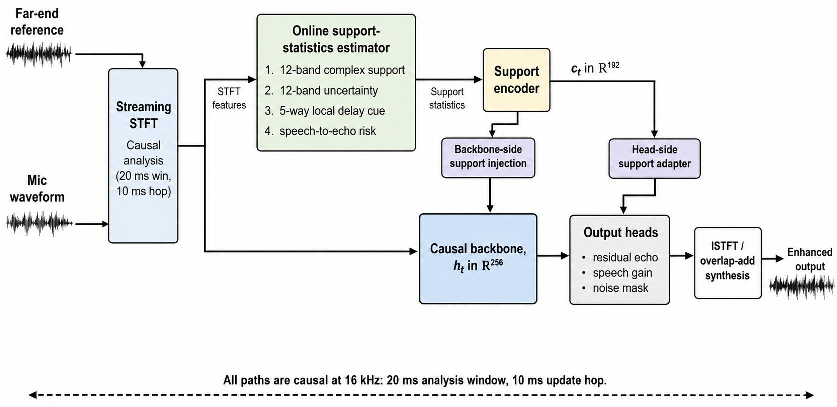
\includegraphics[width=\textwidth]{figures/architecture_overview.pdf}
    \caption{Architecture overview of the support-conditioned streaming AEC family. The evaluated additive and FiLM variants share the same support-statistics front end and backbone-side conditioning path, and differ only in the head-side fusion rule used before the output heads.}
    \label{fig:architecture}
\end{figure*}

\subsection{Low-SER Stress and Family Controls}
The noisy objective table reinforces the same retrained-baseline ordering under a harder public-noise protocol.

\begin{table}[!t]
\caption{Objective results on the harmonized 16 kHz noisy protocol. Public checkpoint transfer rows are moved to appendix audit tables because they are not primary baselines under this contract.}
\label{tab:noisy-main}
\centering
\scriptsize
\begin{tabular}{@{}lrrrr@{}}
\hline
System & SI-SDR (dB) & SegSNR (dB) & ERLE (dB) & RTF \\
\hline
SC-AEC-Echo & 6.94 & 7.28 & 4.80 & 0.30 \\
ASTWS-H16k~\cite{zhao2024astws} & \textbf{9.08} & \textbf{9.22} & \textbf{6.74} & 0.10 \\
NLMS & -20.31 & -11.45 & -13.93 & \textbf{0.07} \\
\hline
\end{tabular}
\end{table}


On the matched noisy split, ASTWS-H16k reaches 9.08~dB SI-SDR, versus 6.94~dB for SC-AEC-Echo. Table~\ref{tab:low-ser-main} adds the 152-example low-SER double-talk slice. These paper-level results make the intrusive evidence a fairness-corrected comparison boundary rather than a single-method victory claim.

\begin{table}[!t]
\caption{Low-SER double-talk stress slice under the harmonized 16 kHz protocol. The zero-conditioning row is a family control; public checkpoint transfer rows are moved to appendix audit tables.}
\label{tab:low-ser-main}
\centering
\scriptsize
\begin{tabular}{@{}lrrrr@{}}
\hline
System & SI-SDR (dB) & SegSNR (dB) & DT-pres. & DT-supp. (dB) \\
\hline
SC-AEC-Echo & 3.10 & 4.75 & 0.050 & 1.48 \\
ASTWS-H16k~\cite{zhao2024astws} & \textbf{7.57} & 8.03 & \textbf{0.030} & \textbf{5.67} \\
NLMS & -19.47 & -10.45 & 0.220 & -9.08 \\
SC-AEC-NoCond & -6.83 & -- & 0.063 & -0.47 \\
\hline
\end{tabular}
\end{table}


The low-SER slice is the sharper overlap test. ASTWS-H16k reaches 7.57~dB SI-SDR, while SC-AEC-Echo reaches 3.10~dB. Relative to SC-AEC-NoCond, SC-AEC-Echo improves signal-to-distortion ratio by 9.93~dB, reduces double-talk preservation error by 0.0133, and improves double-talk suppression by 1.95~dB. This is family-level evidence that support conditioning prevents the zero-conditioning collapse; it is not evidence that each cue has been individually identified as causal.

\subsection{Conditioning-Family Evidence}
The family ablation holds the objective and data pipeline fixed while changing only the conditioning rule. The table should be read as within-family evidence: removing or weakening the conditioning path materially hurts performance, even though the paper does not claim that one cue or one fusion location is already a complete mechanistic explanation.

\begin{table}[!t]
\caption{Conditioning-family diagnostic under the harmonized clean and low-SER protocol.}
\label{tab:ablation-main}
\centering
\scriptsize
\begin{tabular}{lrrrr}
\hline
Variant & Clean & Low-SER & DT supp. & RTF \\
\hline
Additive head fusion & 7.55 & 3.10 & 1.48 & 0.28 \\
FiLM head fusion & 7.26 & 2.79 & 1.41 & 0.30 \\
Zero-conditioning control & -0.51 & -6.83 & -0.47 & 0.46 \\
\hline
\end{tabular}
\end{table}


These results establish only a family-level conditioning effect. Across the evaluated variants, explicit conditioning moves the model away from the collapsed zero-conditioning regime. Because SC-AEC-NoCond is unusually weak, the table should not be read as a complete mechanism proof or as cue-wise attribution. Instead, it shows that this lightweight SC-AEC backbone is structurally reliant on an explicit conditioning path under the evaluated contract; in this family, conditioning acts as a mandatory structural stabilizer rather than as proof of a general control principle.

\begin{table}[!t]
\caption{Gate B cue-attribution controls on 32-example clean, low-SER, and noisy probes. The all-cues row does not beat random or shuffled support on noisy SI-SDR, and removing individual cues does not produce meaningful degradation, so these controls do not establish cue-specific causality.}
\label{tab:gate-b-cue-attribution}
\centering
\scriptsize
\begin{tabular}{lrrrl}
\hline
Variant & Clean & Low-SER & Noisy & Role \\
\hline
All cues & 7.25 & 3.49 & 7.21 & all-cue baseline \\
No complex support & 7.30 & 3.57 & 7.25 & control \\
No uncertainty & 7.27 & 3.46 & 7.25 & control \\
No delay & 7.28 & 3.56 & 7.26 & control \\
No risk cue & 7.27 & 3.55 & 7.25 & control \\
Random support & 7.26 & 3.56 & 7.27 & control \\
Shuffled support & 7.31 & 3.60 & 7.28 & control \\
Stale support & 7.21 & 3.45 & 7.18 & control \\
\hline
\end{tabular}
\end{table}


The Gate B controls close that mechanism boundary. The all-cues continuation reaches 7.25/3.49/7.21~dB clean/low-SER/noisy SI-SDR on the 32-example probes, but random support reaches 7.26/3.56/7.27~dB and shuffled support reaches 7.31/3.60/7.28~dB. Removing individual cues also does not cause meaningful degradation: no-complex-support, no-delay, no-speech-to-echo-risk, and no-uncertainty variants remain within the same narrow band. These negative controls mean the current $\mu/u/d/\rho$ cue design does not establish cue-specific causality; at most, the present family shows that this backbone benefits from a conditioning path under this recipe.

\subsection{Blind AECMOS as Diagnostic Coordinate}
The blind result is a diagnostic cross-system comparison rather than a single global ranking. SC-AEC-Echo occupies the echo-oriented end of the evaluated set, but that position is treated as an unsafe standalone coordinate because the same no-reference metric rewards degenerate silence.

\begin{table}[t]
\caption{Diagnostic validation suite (non-blind synthetic controls) for AECMOS anti-gaming. Degenerate silence receives high scores, so AECMOS is used only with retention, dropout, and listening diagnostics.}
\label{tab:aecmos-controls}
\centering
\small
\begin{tabular}{lrr}
\hline
System & AECMOS-Echo & AECMOS-Other \\
\hline
SC-AEC-Echo & 4.45 & 2.18 \\
Mic pass & 2.14 & 3.94 \\
Attenuated mic & 2.14 & 3.94 \\
All-zero & 4.65 & 4.97 \\
\hline
\end{tabular}
\end{table}

\begin{table}[!t]
\caption{Official ICASSP 2023 blind-set AECMOS (doubletalk + far-end single-talk).}
\label{tab:blind-aecmos}
\centering
\begin{tabular}{lrr}
\hline
System & Echo & Other \\
\hline
SC-AEC-Echo & 4.08 & 3.54 \\
ASTWS-H16k~\cite{zhao2024astws} & 3.58 & 3.71 \\
NLMS & 3.01 & 4.06 \\
ASTWS transfer~\cite{zhao2024astws} & 2.43 & 4.43 \\
Deep Echo transfer~\cite{zhao2024deepecho} & 3.30 & 4.02 \\
\hline
\end{tabular}
\end{table}

\input{generated/taslp_blind_retention_table.tex}

Table~\ref{tab:aecmos-controls} is the no-reference integrity check used before interpreting blind coordinates. Fig.~\ref{fig:blind-summary} then shows the corresponding no-reference echo/non-echo split together with the microphone-active dropout diagnostic.

\begin{figure}[t]
    \centering
    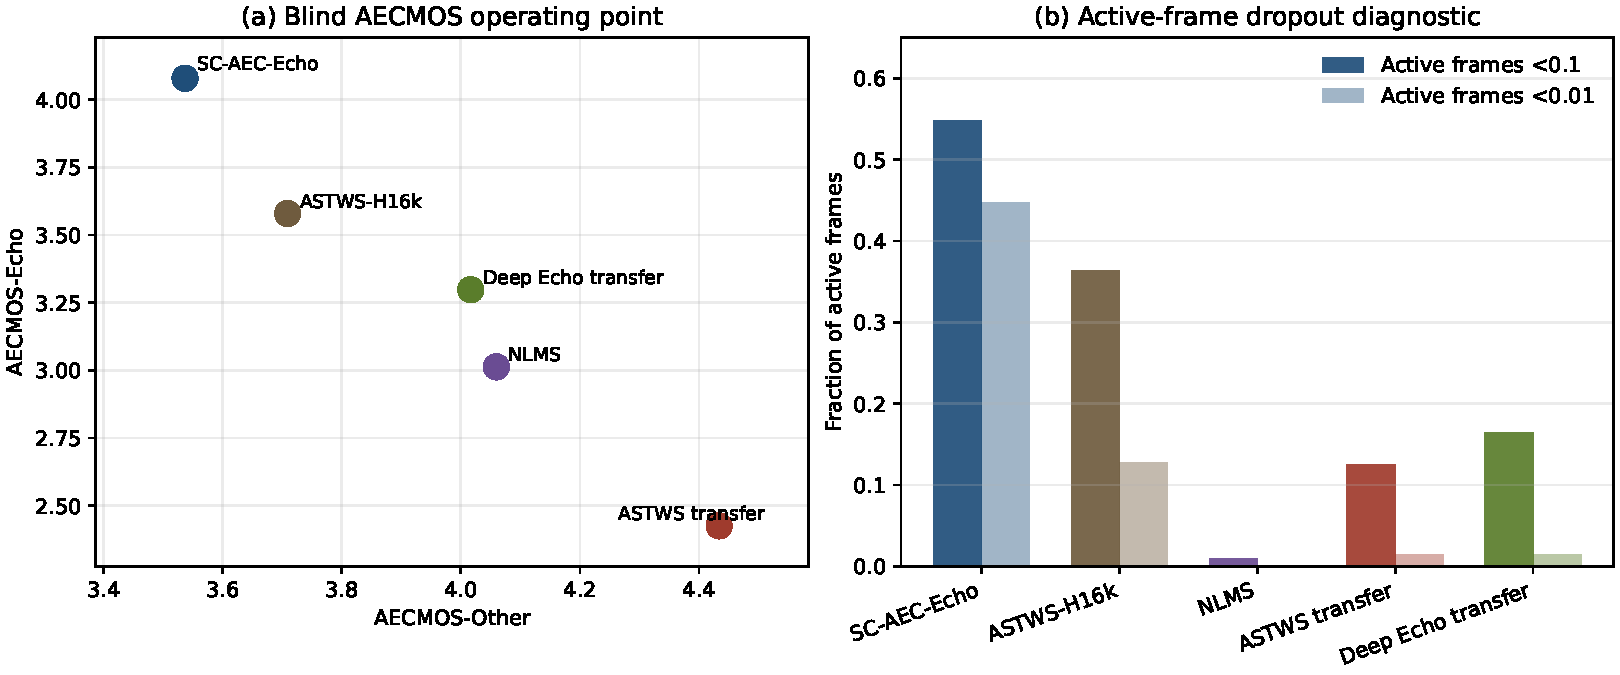
\includegraphics[width=\columnwidth]{figures/taslp_blind_summary.pdf}
    \caption{Blind AECMOS and retention summary. Left: overall no-reference AECMOS coordinate. Right: microphone-active frame dropout on the shared blind double-talk subset. AECMOS is used only as a diagnostic coordinate because validation controls show that degenerate outputs can receive high AECMOS scores.}
    \label{fig:blind-summary}
\end{figure}

The scenario split explains the tradeoff. In blind double-talk, SC-AEC-Echo reaches an echo coordinate of 4.43 versus 4.06 for ASTWS-H16k, while ASTWS-H16k retains a higher non-echo coordinate of 2.42 versus 2.08 for SC-AEC-Echo. In blind far-end single-talk, the non-echo axis is effectively saturated for all systems while SC-AEC-Echo retains a higher echo coordinate of 3.73 versus 3.10 for ASTWS-H16k. Overall, SC-AEC-Echo occupies a higher blind echo coordinate than ASTWS-H16k by 0.50 with 95\% CI $[0.45,0.55]$, while ASTWS-H16k occupies a higher complementary non-echo coordinate than SC-AEC-Echo by 0.17 in magnitude with 95\% CI $[0.13,0.21]$. Because Table~\ref{tab:aecmos-controls} shows that all-zero output scores 4.65/4.97, this AECMOS-Echo difference is not perceptual evidence by itself.

The frame-level retention analysis on the 82 shared blind double-talk clips shows a much more aggressive operating point: SC-AEC-Echo keeps a clip-level RMS ratio of 0.62 on average, but drives 54.8\% of active frames below a 0.1 microphone-RMS ratio, versus 36.4\% for ASTWS-H16k and 12.5\% for the ASTWS public-checkpoint transfer row. The all-zero validation control in Table~\ref{tab:aecmos-controls} also receives implausibly high AECMOS values (Echo 4.65, Other 4.97). The blind echo score is therefore reported together with retention diagnostics rather than treated as standalone perceptual evidence.

\subsection{Returned Item-Level Listening Summaries}

\begin{table*}[t]
\caption{Returned 72-base item-level listening summaries including ASTWS-H16k. Values are means with 95\% bootstrap confidence intervals over base clips/items; raw individual-rater rows are unavailable, and overlapping intervals make these descriptive boundary summaries rather than a formal listener-preference ranking. Higher is better for all columns.}
\label{tab:returned-human}
\centering
\footnotesize
\begin{tabular}{lrrrrr}
\hline
System & Items & Overall MOS & Echo MOS & Near-end MOS & Accept rate \\
\hline
ASTWS-H16k & 72 & 3.73 [3.54, 3.93] & 4.14 [3.92, 4.33] & 3.51 [3.25, 3.75] & 0.71 [0.60, 0.81] \\
SC-AEC-Preserve & 72 & 3.46 [3.27, 3.66] & 4.13 [3.93, 4.31] & 3.06 [2.80, 3.31] & 0.57 [0.46, 0.69] \\
SC-AEC-Echo & 72 & 3.34 [3.14, 3.54] & 4.16 [3.97, 4.35] & 2.92 [2.63, 3.20] & 0.53 [0.42, 0.64] \\
NLMS & 72 & 3.45 [3.24, 3.67] & 3.76 [3.54, 3.99] & 3.28 [3.00, 3.57] & 0.53 [0.42, 0.65] \\
ASTWS transfer & 72 & 3.39 [3.21, 3.57] & 3.00 [2.72, 3.28] & 4.11 [3.97, 4.25] & 0.53 [0.42, 0.64] \\
Deep Echo transfer & 72 & 3.60 [3.40, 3.79] & 3.90 [3.67, 4.10] & 3.42 [3.15, 3.68] & 0.62 [0.51, 0.74] \\
\hline
\end{tabular}
\end{table*}

\begin{table*}[t]
\caption{Returned item-level listening-summary scenario split for overlap-heavy and near-end single-talk cases. Each scenario cell reports O/N, where O is overall MOS and N is near-end naturalness MOS; rows use the same item-level summaries as Table~\ref{tab:returned-human}.}
\label{tab:returned-human-scenario}
\centering
\footnotesize
\begin{tabular}{lrrrr}
\hline
System & Double-talk O/N & Low-SER O/N & Noisy DT O/N & Near-end ST O/N \\
\hline
ASTWS-H16k & 3.78/3.28 & 3.13/2.35 & 3.60/2.88 & 4.22/3.41 \\
SC-AEC-Preserve & 3.54/2.86 & 2.78/1.97 & 3.03/2.17 & 4.40/3.71 \\
SC-AEC-Echo & 3.64/3.01 & 2.53/1.64 & 2.97/2.04 & 4.41/3.73 \\
NLMS & 3.50/3.19 & 2.69/2.09 & 2.67/2.02 & 4.39/3.68 \\
ASTWS transfer & 3.69/3.93 & 3.19/3.84 & 3.10/3.73 & 4.44/3.76 \\
Deep Echo transfer & 3.47/3.27 & 2.90/2.10 & 3.31/2.56 & 4.39/3.68 \\
\hline
\end{tabular}
\end{table*}


The returned 72-base item-level listening summaries are the main perceptual boundary for this revision. Table~\ref{tab:returned-human} does not support an overall human win for any SC-AEC operating point. ASTWS-H16k has the highest returned item-level mean overall MOS and acceptability in this returned summary. Its returned item-level means are 3.73 for overall MOS and 0.71 for acceptability, while SC-AEC-Preserve reaches 3.46 overall MOS and SC-AEC-Echo reaches 3.34. SC-AEC-Echo is close to ASTWS-H16k on echo-annoyance MOS (4.16 versus 4.14), but its near-end naturalness remains lower (2.92 versus 3.51), so the echo-oriented coordinate still does not translate into a better overall listening point. Because the returned summaries are item-level and several confidence intervals overlap, these values are used as perceptual boundary evidence rather than as a formal listener-preference ranking. SC-AEC-Preserve has the highest returned item-level mean among SC-AEC rows on overall MOS, near-end naturalness, and acceptability, but the 3.46 versus 3.34 overall-MOS gap between SC-AEC-Preserve and SC-AEC-Echo has overlapping confidence intervals and should not be read as a robust perceptual separation.

The scenario summary localizes the remaining limitation. Table~\ref{tab:returned-human-scenario} shows that overlap-heavy cases remain the main pressure point: low-SER and noisy double-talk lower near-end naturalness for every nonlinear system, and SC-AEC-Echo remains especially aggressive on those slices. The near-end single-talk column is included as a preservation anchor: it shows that most systems recover higher near-end naturalness when echo overlap is absent, which makes the overlap limitation harder to dismiss as a global rating artifact. The worst SC-AEC clips are dominated by over-gating, dropouts, level pumping, large silence fractions, and bandwidth or tonal artifacts. The returned human evidence therefore converts the earlier preservation concern into a concrete limitation: echo-side coordinates are not enough unless a preservation point also survives overlap naturalness checks.

The NLMS row is an important diagnostic rather than a throwaway baseline. NLMS remains perceptually competitive despite very poor objective SI-SDR in the matched reconstruction tables. The NLMS objective rows are not presented as evidence of strong intrusive reconstruction; they show the opposite. Their value is diagnostic: poor target-matched SI-SDR can still coexist with acceptable listener preference when the output avoids neural dropouts, level pumping, and tonal artifacts. Mechanistically, the extreme negative ERLE/SI-SDR values on synthetic matched sets occur when this simple linear wrapper is exposed to uncompensated temporal shifts, non-causal mixture artifacts, and double-talk without explicit protection, causing the adaptive path to misalign under the target-reconstruction contract. The returned listening summaries, which are anchored by stable rendered clips rather than this synthetic reconstruction objective alone, therefore show why a linear path can remain perceptually competitive even when intrusive synthetic metrics reject it. For streaming AEC, avoiding artificial degradation can matter more than maximizing an echo-side no-reference coordinate.

\section{Discussion}
The objective and blind results tell a coherent story once the result boundary is explicit. Under one harmonized objective protocol, ASTWS-H16k is stronger on intrusive clean, noisy, and low-SER SI-SDR. Under blind evaluation, SC-AEC-Echo enters a more aggressive echo-removal regime, which raises the echo-oriented coordinate while paying a non-echo and retention penalty concentrated in double-talk.

This cross-system comparison trades echo suppression against model size and near-end preservation. SC-AEC-Echo is materially heavier than the compact public baselines, and the blind frame-level analysis shows that it is materially more aggressive during overlap. The returned item-level listening summaries sharpen that picture: SC-AEC-Preserve shifts within the SC-AEC family, but it does not close the listening-summary gap to ASTWS-H16k, and its overall MOS is too close to SC-AEC-Echo to support a robust preference claim. The preservation-biased point is therefore a boundary point in the diagnostic protocol, not a promoted preferred system.

The AECMOS result is useful precisely because it becomes unsafe when isolated. AECMOS was designed to separate echo impairment from other degradation, but the all-zero validation control (Echo 4.65, Other 4.97) and microphone-active retention table show why a blind no-reference score cannot be used without anti-gaming diagnostics. The paper therefore treats AECMOS as a diagnostic coordinate, not as a replacement for listening or as standalone positive evidence for SC-AEC.

The cue-control result has a methodological implication. The conditioning path stabilizes this recurrent suppressor, but destructive random and shuffled support controls prevent attributing the effect to the individual $\mu/u/d/\rho$ cues. For future conditioned AEC systems, a metric-positive operating point should therefore be accompanied by destructive cue controls before a mechanism claim is made. ASTWS-H16k also succeeds under the same data and evaluation contract, so the harmonized objective itself is not the limiting factor.

That distinction matters for future work. The remaining problem is not simply ``suppress harder.'' The unresolved question is preservation-aware control under motion and far-end single-talk: a system must preserve near-end speech and avoid artificial dropouts while still suppressing echo in low-SER overlap. The NLMS result is a useful reminder that a simple linear filter can remain perceptually competitive when it avoids neural artifacts.

The baseline-fidelity evidence should be interpreted with equal care. Native-compat forward matching rules out a simple wrapper bug on the probe manifest, but it does not prove full equivalence to every native training or evaluation choice made by the baseline authors. The ASTWS-H16k result shows that the ASTWS architecture can be competitive under the harmonized recipe when retrained, so the public-checkpoint collapse is not used as positive comparison evidence.

\section{Limitations}
The blind no-reference metric remains a surrogate rather than a standalone perceptual oracle. The diagnostic validation suite also shows that the ONNX backend can assign implausibly high scores to all-zero controls, so the blind AECMOS results should be treated as comparative operating-point evidence rather than human validation.

The present manuscript is also narrow on mechanism. The ablations demonstrate a family-level conditioning effect under one fixed objective, but Gate B does not isolate the contribution of each support statistic or establish a full causal mechanism for any cue. The zero-conditioning control is a collapse diagnostic, not a complete capacity-matched proof. The 0--4~ms delay cue is also only a local alignment statistic; it is not a robust device-delay estimator, and delay-offset or echo-path-motion stress tests are needed before treating it as deployment evidence. The paper therefore avoids claiming that one specific cue, fusion location, or operating-point heuristic is a general principle beyond the currently evaluated family.

The returned human evidence is item-level rather than raw rater-level. The ASTWS-H16k-inclusive returned artifact covers 432 formal presentations and includes package QC repeats and traps, but it does not expose individual rater rows or listener-level screening records. The resulting table is sufficient to narrow the claim, but not to claim a formal P.808 ranking.

Finally, the paper reports only fixed diagnostic points, not a swept Pareto curve. The results show that the evaluated family exposes a family-level echo-removal response, but its preservation side needs a materially different method direction, stronger controlled ablations, and a larger fresh listening evaluation before any human-preference claim would be justified.

\section{Availability and Reproducibility}
All tables and figures are generated from fixed artifacts. The supplementary reproducibility material for review contains the manifest definitions, evaluation scripts, table-generation scripts, fixed result summaries, baseline-fidelity audit artifacts, and returned item-level listening summaries used by the manuscript. It also contains the fixed 72-base listening-summary material and returned-rating ingest scripts. When official challenge audio cannot be redistributed directly, the material includes reconstruction instructions rather than raw audio mirrors.

Auxiliary literature notes are not part of the evidence record.

\section{Conclusion}
We introduced a multi-axis anti-gaming evaluation protocol for streaming acoustic echo cancellation and demonstrated its practical necessity with a support-conditioned causal AEC probe. Under one harmonized 16~kHz protocol, retraining the public ASTWS architecture under the same data and evaluation contract is stronger on intrusive clean, noisy, and low-SER SI-SDR than SC-AEC-Echo. On the official blind set, SC-AEC-Echo occupies a higher echo-oriented no-reference coordinate while revealing a clear non-echo and retention tradeoff in double-talk, but the all-zero AECMOS validation control prevents using that coordinate as standalone perceptual evidence. Returned 72-base item-level listening summaries that include ASTWS-H16k indicate that this echo-oriented coordinate has not translated into the strongest returned item-level overall-MOS or acceptability point: ASTWS-H16k has the highest returned item-level mean overall MOS and acceptability in this returned summary, while the ASTWS public-checkpoint transfer row has the highest returned item-level mean near-end naturalness.

The resulting conclusion is therefore specific. The evaluated family exposes a family-level echo-removal response, but the present evidence does not isolate cue-specific causal mechanisms and the current family has not solved near-end preservation or objective competitiveness against a retrained modern public architecture. We argue that standard AEC evaluation should be expanded into a multidimensional diagnostic framework: intrusive SI-SDR for target reconstruction, no-reference AECMOS only with mandatory microphone-active retention and dropout anti-gaming checks, and returned or newly collected perceptual anchors including classical baselines. Without all three axes, a single metric can reward the wrong diagnostic point.

\appendices
\section{Baseline Fidelity and Historical Anchor}
\label{app:fidelity}
\par\noindent
\refstepcounter{table}
\label{tab:historical-anchor}
\begin{center}
\textbf{TABLE \thetable}\\
\parbox{0.96\linewidth}{\centering Historical clean anchor reported outside the main runnable-baseline claim.}\\[0.5ex]
\scriptsize
\begin{tabular}{@{}lrrr@{}}
\hline
System & SI-SDR (dB) & SegSNR (dB) & ERLE (dB) \\
\hline
SC-AEC-Echo & 7.55 & 7.71 & 5.22 \\
ICASSP 2022~\cite{cutler2022aec} & 9.60 & 6.38 & 3.90 \\
\hline
\end{tabular}
\end{center}
\par\medskip

\par\noindent
\refstepcounter{table}
\label{tab:baseline-fidelity}
\begin{center}
\textbf{TABLE \thetable}\\
\parbox{0.96\linewidth}{\centering Baseline-fidelity summary. The reported column is context only, not a same-protocol comparison.}\\[0.5ex]
\scriptsize
\begin{tabular}{lrrr}
\hline
System & Reported & Native probe & Shared clean \\
\hline
ASTWS transfer~\cite{zhao2024astws} & 23.46 & -0.45 & -0.89 \\
Deep Echo transfer~\cite{zhao2024deepecho} & 19.85 & 1.80 & 1.83 \\
ICASSP 2022~\cite{cutler2022aec} & -- & -- & 9.60 \\
\hline
\end{tabular}
\end{center}
\par\medskip

\par\noindent
\refstepcounter{table}
\label{tab:baseline-audit}
\begin{center}
\textbf{TABLE \thetable}\\
\parbox{0.96\linewidth}{\centering Compact baseline-fairness audit on one clean probe pack and one low-SER stress probe pack. Native-compat forward and the corrected wrapper are compared under the same diagnostic manifests.}\\[0.5ex]
\scriptsize
\begin{tabular}{llrrrr}
\hline
Subset & System & Native & Wrapper & $\Delta$SI & $\Delta$DT \\
\hline
Clean probe & ASTWS transfer & -0.45 & -0.45 & 0.00 & 0.00 \\
Clean probe & Deep Echo transfer & 1.80 & 1.80 & 0.00 & 0.00 \\
Low-SER probe & ASTWS transfer & -7.57 & -7.57 & 0.00 & 0.00 \\
Low-SER probe & Deep Echo transfer & -5.31 & -5.31 & 0.00 & 0.00 \\
\hline
\end{tabular}
\end{center}
\par


The ICASSP~2022 row is reported separately because it is useful historical context but not part of the current runnable-modern-baseline comparison boundary. The fidelity table reports representative native numbers only as context for the evaluation-gap surface; they are not used as same-protocol comparison rows.

The key implementation-audit result is narrow but important. On the 128-example diagnostic clean probe, and again on the 152-example low-SER stress probe, the native-compat forward path and the corrected wrapper produce identical ASTWS public-checkpoint transfer and Deep Echo public-checkpoint transfer waveforms and matched summary metrics. That makes implementation mismatch unlikely as the source of the harmonized baseline gap on those audited probes. It does not, however, prove equality to every native training recipe, sample-rate path, or evaluation convention used by the original authors.

The harmonized clean table is therefore the shared-contract comparison used for the journal claim. The native-report column is included only to show how far a shared re-evaluation can sit from the original public numbers, and why the main text keeps the comparison boundary explicit.

\section{Statistical Reporting Summary}
\label{app:stats}
\begin{table*}[t]
\caption{Statistical reporting summary. All p-values come from paired two-sided sign tests on matched examples; 95\% confidence intervals are bootstrap intervals over the paired mean improvement; Holm correction is applied within each result family.}
\label{tab:stats-summary}
\centering
\scriptsize
\begin{tabular}{p{0.12\textwidth}p{0.07\textwidth}p{0.28\textwidth}p{0.10\textwidth}rll}
\hline
Evidence role & Family & Comparison & Metric & Mean effect & 95\% CI & Holm-corrected $p$ \\
\hline
paper-level & Clean & SC-AEC-Echo vs ASTWS-H16k & SI-SDR (dB) & -4.16 & [-4.35, -3.97] & 6.73e-109 \\
paper-level & Noisy & SC-AEC-Echo vs ASTWS-H16k & SI-SDR (dB) & -2.14 & [-2.36, -1.92] & 7.41e-48 \\
paper-level & Low-SER & SC-AEC-Echo vs ASTWS-H16k & SI-SDR (dB) & -4.47 & [-4.78, -4.16] & 2.05e-40 \\
paper-level & Blind & SC-AEC-Echo vs ASTWS-H16k & AECMOS-Echo & 0.50 & [0.45, 0.55] & 3.70e-68 \\
paper-level & Blind & SC-AEC-Echo vs ASTWS-H16k & AECMOS-Other & -0.17 & [-0.21, -0.13] & 4.80e-28 \\
family ablation & Low-SER & SC-AEC-Echo vs SC-AEC-NoCond & DT suppression (dB) & 1.95 & [1.62, 2.29] & 4.33e-19 \\
family ablation & Low-SER & SC-AEC-Echo vs SC-AEC-NoCond & DT preservation & 0.01 & [0.01, 0.02] & 3.97e-21 \\
family ablation & Low-SER & SC-AEC-Echo vs SC-AEC-NoCond & SI-SDR (dB) & 9.93 & [9.42, 10.44] & 1.61e-43 \\
classical diagnostic & Blind & SC-AEC-Echo vs NLMS & AECMOS-Echo & 1.07 & [0.98, 1.15] & 3.93e-82 \\
classical diagnostic & Blind & SC-AEC-Echo vs NLMS & AECMOS-Other & -0.52 & [-0.58, -0.47] & 1.24e-63 \\
transfer audit & Clean & SC-AEC-Echo vs Deep Echo transfer & SI-SDR (dB) & 5.72 & [5.30, 6.12] & 9.46e-71 \\
transfer audit & Noisy & SC-AEC-Echo vs Deep Echo transfer & SI-SDR (dB) & 6.34 & [5.96, 6.70] & 1.03e-119 \\
transfer audit & Blind & SC-AEC-Echo vs ASTWS transfer & AECMOS-Echo & 1.65 & [1.58, 1.72] & 4.00e-139 \\
transfer audit & Blind & SC-AEC-Echo vs ASTWS transfer & AECMOS-Other & -0.90 & [-0.98, -0.81] & 1.70e-128 \\
transfer audit & Blind & SC-AEC-Echo vs Deep Echo transfer & AECMOS-Echo & 0.78 & [0.72, 0.84] & 1.38e-92 \\
transfer audit & Blind & SC-AEC-Echo vs Deep Echo transfer & AECMOS-Other & -0.48 & [-0.55, -0.41] & 2.04e-55 \\
\hline
\end{tabular}
\end{table*}


\section{Blind Validation and Supplementary Perceptual Details}
\label{app:aecmos-validation}
As shown in Table~\ref{tab:blind-retention} in the main text, SC-AEC-Echo is materially more aggressive than ASTWS-H16k and the public-checkpoint transfer rows on microphone-active overlap frames. The supplementary tables below therefore treat AECMOS as a surrogate coordinate rather than as standalone perceptual evidence.
\par\noindent
\refstepcounter{table}
\label{tab:synthetic-aecmos}
\begin{center}
\textbf{TABLE \thetable}\\
\parbox{0.96\linewidth}{\centering Supplementary synthetic AECMOS on clean and low-SER sets.}\\[0.5ex]
\begin{tabular}{llrr}
\hline
Suite & System & Echo & Other \\
\hline
Low-SER & SC-AEC-Echo & 4.30 & 2.03 \\
Low-SER & ASTWS transfer~\cite{zhao2024astws} & 2.26 & 3.90 \\
Low-SER & Deep Echo transfer~\cite{zhao2024deepecho} & 3.63 & 2.37 \\
Clean & SC-AEC-Echo & 4.30 & 2.62 \\
Clean & ASTWS transfer~\cite{zhao2024astws} & 2.44 & 3.99 \\
Clean & Deep Echo transfer~\cite{zhao2024deepecho} & 3.87 & 2.69 \\
\hline
\end{tabular}
\end{center}
\par\medskip

\paragraph{AECMOS validation check.}
The ONNX AECMOS backend is used as a comparative signal only. The validation suite returned status \texttt{warning}, and the all-zero control still receives implausibly strong echo or non-echo scores.


\bibliographystyle{IEEEtran}
\bibliography{refs}

\end{document}
